%\section{Introduction}
Conducting a literature review is an essential step in any research project. In this section, we reviewed research papers related to the internship's topics, including code refactoring for improving software energy efficiency and genetic improvement for getting better versions of software. Through this review, we assessed the strengths and limitations of the existing research. 

\vspace{.5em}
The insights gained from this review were in identifying potential code refactoring techniques for improving software energy efficiency, this answering RQ2.

\section{Code Refactoring for Software Energy Efficiency}
%In this section, we will review the existing research on code refactoring, exploring its significance and advantages. Additionally, we will investigate various available code refactoring techniques, conducting a comparative analysis to identify the most suitable code refactoring techniques. Subsequently, we will select the suitable code refactoring techniques for integration into the gin tool, based on the findings of our comparison. 

%\subsection{Code Refactoring}

Code refactoring is the process of restructuring existing computer code without changing its external behavior to enhance reusability and maintainability of software.
%components through improving nonfunctional attributes of the software ~\cite{DBLP:journals/cluster/KimHYL18}. It is a way to improve the code quality and maintainability\footnote{\url{https://www.c-sharpcorner.com/article/pros-and-cons-of-code-refactoring/}}. 
The benefits of code refactoring include removing bad smells, reducing code size, improving readability, and making it easier to enhance and maintain in the future. However,
the main limitations of applying code refactoring is that could be time expensive and error-prone. So, its automatising is crucial for supporting developers and architects. 
%there are also limitations to code refactoring. For example, it can be time consuming and 
%expensive and risky in the view of management, may introduce bugs, and can be difficult to do if the code is already a big mess. Additionally, refactoring should not be done if a deadline is near or if the cost of refactoring is higher than rewriting the code from scratch\footnotemark[1]. 

\vspace{.5em}
In the context of energy efficiency, code refactoring can be used to improve the energy consumption of software by making changes to the source code that reduce its energy usage. Several studies have investigated the impact of code refactoring on energy consumption (see Table~\ref{tab:comparison} that presents three main studies in this domain). 

\cite{DBLP:conf/esem/SahinPC14} presented an empirical study to investigate the energy impacts of 197 applications using 6 commonly-used code refactoring methods, for instance \texttt{Convert Local Variable to Field} (see Row 1 in Table~\ref{tab:comparison}). The results show that code refactoring methods can not only impact energy usage but can also increase and decrease the amount of energy used by an application. 

%Another study~\cite{DBLP:conf/icsoft/OurnaniRRP21a} found that developers can optimize the power consumption of software by improving their source code implementations. 
\cite{DBLP:journals/tse/MoralesSKCA18} proposed a code smell or anti-pattern correction approach called EARMO. EARMO is a multi-objective search based technique that improves energy efficiency and the quality of code by using code refactoring. In this study, the researchers analyzed the impact of eight types of anti-patterns, for instance \texttt{Move Method} that refactors the \texttt{Bob (God class)} code smell (see Row 2 in Table~\ref{tab:comparison}).
%on a testbed of 20 android apps extracted from F-Droid and evaluated EARMO using three multi-objective search-based algorithms. 
%The results showed that 
EARMO is able to
%can generate refactoring recommendations in less than a minute and 
remove a median of 84\% of code smells or anti-patterns. Moreover, EARMO extended the battery life of a mobile phone by up to 29 minutes. 
%when running a refactored multimedia app with default settings (no Wi-Fi, no location services, and minimum screen brightness) in isolation. 
%A qualitative study was also conducted with developers of the studied apps to assess the refactoring recommendations made by EARMO. 
An experiment with developer showed that EARMO suggest 68\% of code refactoring  are relevant for improving the quality of code and energy efficiency. 
%suggested by EARMO to be very relevant. 
%Additionally, code smells, which are symptoms of poor design or implementation choices, have been found to impact energy consumption. 

\cite{DBLP:journals/infsof/PalombaNPZL19} founded that code refactoring for android applications, for instance refactoring the \texttt{Data Transmission Without Compression} code smell (see Row 3 in Table~\ref{tab:comparison}), is able to reduced energy consumption by up to 10.8\%. Moreover, four code smells increase method energy consumption by up to 87 times.


\begin{table}[!h]
\centering
\scalebox{0.8}{
\begin{tabular}{|p{3.5cm}|p{6.5cm}|p{5cm}|p{2cm}|p{2cm}|}

\hline
\textbf{Reference} & \textbf{Code refactoring} & \textbf{Experiment / Bench-marking} & \textbf{Tool for EC} & \textbf{Results}  \\

\hline
\cite{DBLP:conf/esem/SahinPC14} & 
\textbf{Code refactoring (6)}: Convert Local Variable to Field,
Extract Local Variable,
Extract Method,
Introduce Indirection, 
Inline Method
Introduce Parameter Object & 
9 Java Applications (ex. cMath, cCollections, ..) & 
Low Power Energy Aware Process (LEAP) & 
-7.50\% to 4.54\%  \\
\hline

\cite{DBLP:journals/tse/MoralesSKCA18} & 
\textbf{Android code smells (3)}: Binding resources too early class, Private getter and setters, HashMap usage. \textbf{OO code smells (5)}: Lazy class, Blob (God class), Long-parameter list, Refused bequest, Speculative Generality & 
\textbf{Phase 1:} Empirical Study to understand in which extent 8 code refactorings help to save energy. 
\textbf{Phase 2:} EARMO is developped to select optimal series of code refactoring.  The energy consumed by the version of code is inferred from Phase 1. & 
Not reported. &
EARMO is able to save 29 minutes of battery.
\\
\hline

\cite{DBLP:journals/infsof/PalombaNPZL19} & 
\textbf{Android-specific code smells (9)}: Data Transmission Without Compression, Durable Wakelock, Inefficient Data Structure, Inefficient SQL Query, Inefficient Data Format And Parser, Internal Setter, Leaking Thread,  Member-Ignoring Method, Slow Loop & 
60 Android Java apps (categories ex. games, productivity, social, etc) & 
PETRA (Power Estimation Tool for Android) & 
Four code smell types increase method energy consumption by up to 87 times.
\\
\hline
\end{tabular}
}
\caption{Comparison of approaches}
\label{tab:comparison}
\end{table}

According to the information mentioned above, it can be concluded that code refactoring can have a positive impact on energy efficiency by reducing the energy consumption of software. However, the benefits and limitations of code refactoring for energy efficiency may vary depending on the specific context and implementation.

%\subsection{Types of Code Refactoring Techniques and Comparison between mentioned Code Refactoring Techniques}

\vspace{.5em}
In Table \ref{tab:Types_Code_Refactoring_Techniques}, we present the 
%different types of 
code refactoring techniques studied in the previous works. We introduce them because the authors of these works provided individual information about their positive impact in energy efficiency. So, it provides us more insights about their usefulness in software energy efficiency.
%and compare them based on energy consumption impact 

{\footnotesize
\begin{longtable}{|c|p{2cm}|p{4.3cm}|p{8cm}|}
%\begin{table}[ht!]
%\caption{Types of Code Refactoring Techniques}
%\label{tab:Types_Code_Refactoring_Techniques}
%\scalebox{0.8}{
%\begin{tabular}{|c|p{2cm}|p{4cm}|p{13cm}|}

  \hline
\textbf{Ref.} &  \textbf{Code Refactoring Technique} & \textbf{Purpose} & \textbf{Energy Consumption Impact}\\
  
  \hline
\multirow{6}{*}{\rotatebox[origin=rc]{90}{\cite{DBLP:conf/esem/SahinPC14}}} &
  Convert Local Variable to Field
  %~\cite{DBLP:conf/esem/SahinPC14} 
  & 
  Turns a local variable into a field. &
  This refactoring had a statistically significant difference in energy usage in some cases for JVM. This means that in some cases, applying this refactoring resulted in a noticeable change in the amount of energy used by the program. In most cases, applying this refactoring resulted in an decrease in the amount of energy used by the program.  \\
  
 \cline{2-4}
 & Extract Local Variable
 %~\cite{DBLP:conf/esem/SahinPC14} 
 & 
 Creates a new variable assigned to the selected expression and replaces the selection with a reference to the new variable. &
 It had the least impact on energy usage, with only a few cases showing a significant difference. This means that in most cases, applying this refactoring did not result in a noticeable change in the amount of energy used by the program. In some cases, for JVM 6, the amount of energy used by the program decreases\\
  
 \cline{2-4}
 & Extract Method 
  %~\cite{DBLP:conf/esem/SahinPC14}
  & 
  Creates a new method containing the selected statement or expression and replaces the selection with a reference to the new method. &
  This refactoring increased energy usage 8 times and decreased energy usage 2 times on JVM6. This means that in most cases, applying this refactoring resulted in an increase in the amount of energy used by the program. However, in a few cases, there was a decrease in energy usage after applying this refactoring.\\
  
 \cline{2-4}
 & Inline Method 
  %~\cite{DBLP:conf/esem/SahinPC14} 
  & 
  Copies the body of a called method into the body of a caller method. &
  It had varying impacts on energy usage across different applications and platforms. This means that the impact of this refactoring on energy usage is not consistent and can vary depending on the specific application and platform. In some cases, it may reduce energy usage, while in others it may increase it. \\
  
 \cline{2-4}
 & Introduce Indirection
 %~\cite{DBLP:conf/esem/SahinPC14} 
 & 
 Creates a static method to indirectly delegate to the selected method. &
 This refactoring had both positive and negative impacts on energy usage. This means that the impact of this refactoring on energy usage is not consistent and can vary depending on the specific case. In most cases, applying this refactoring resulted in an increase in the amount of energy used by the program. However, in a few cases, there was a decrease in energy usage after applying this refactoring. \\
  
 \cline{2-4}
 & Introduce Parameter Object
 %~\cite{DBLP:conf/esem/SahinPC14} 
 & 
 Replaces a set of parameters with a new class and updates all callers to pass an instance of the new class as the value to the introduced parameter. &
 It had a significant impact on energy usage. This means that in most cases, applying this refactoring resulted in a decrease in the amount of energy used by the program. \\
 
  \hline 
\multirow{1}{*}{\rotatebox[origin=rc]{90}{\cite{DBLP:conf/seke/ParkHL14}}} & Encapsulate Field  & 
  Set access permissions of a variable by creating getters and setters for the selected field, allowing the field to be accessed and modified only through these methods. This provides better control over the field and can improve the maintainability of the code. &
  This technique can have an impact on energy efficiency, especially when combined with other code refactoring techniques. These combinations can provide significant improvements in energy efficiency. \\
  
 \hline 
\multirow{1}{*}{\rotatebox[origin=rc]{90}{\cite{barack2018effectiveness}}} & Inline Temp
 & 
 Replace all references to a temporary variable with the expression that was assigned to it. This can improve code readability and reduce the number of variables in the code. \vspace{1.5cm} &
 Eliminating temporary variables speeds up the fetching of redundant temporary variables from both the main and cache memories. This approach improves performance and maintains the same level of energy efficiency, which is considered a positive improvement. \\
  
 \hline
\multirow{1}{*}{\rotatebox[origin=rc]{90}{\cite{DBLP:journals/tse/MoralesSKCA18}}}  & Move Method for refactoring the Blob (God class) code smell
   & 
  Improve the organization of code by moving a method to a more appropriate class or object. \vspace{2cm} &
  Can reduce energy consumption by improving the efficiency of the code. \\
  
 \hline 
\multirow{1}{*}{\rotatebox[origin=rc]{90}{\cite{kim2018code}}} & Simplify Nested Loop
  & 
 Reduce the dimensions of multi-dimensional loops. \vspace{2cm} &
 Dimension reduction of multi-dimensional loops helps to reduce energy consumption and make the code more readable and energy-efficient. \\
  

 \hline
\caption{Types of Code Refactoring Techniques}
\label{tab:Types_Code_Refactoring_Techniques}
\end{longtable}
}
%\end{tabular}}
%\end{table}

%\subsection{Analysis and Selection of Code Refactoring Methods for Integration into the Gin Tool}

%The analysis of various code refactoring techniques, as presented in the table \ref{tab:Types of Code Refactoring Techniques}, reveals distinct patterns in their impact on energy consumption. Several techniques,  including 
From Table~\ref{tab:Types_Code_Refactoring_Techniques}, we can observe that \texttt{Convert Local Variable to Field}, \texttt{Introduce Parameter Object}, \texttt{Inline Temp}, \texttt{Move Method}, \texttt{Simplify Nested Loop} and \texttt{Encapsulate Field}, consistently show positive results in reducing energy consumption across different scenarios. 
%
%Moreover, the combined application of \texttt{Inline Temp}, \texttt{Simplify Nested Loop}, and \texttt{Encapsulate Field} code refactoring techniques proves to be particularly effective in enhancing energy efficiency ~\cite{csanlialp2022energy}.
%
%\vspace{.5em}
Conversely, \texttt{Extract Local Variable}, \texttt{Extract Method}, \texttt{Inline Method}, and \texttt{Introduce Indirection} exhibit varying effects on energy consumption depending on the specific context. Hence, it is essential to apply these techniques with caution and consider the unique circumstances of each code-base.

\vspace{.5em}
For integrating code refactoring techniques into the
a genetic improvement method %Gin Tool 
for improving software energy efficiency, we can consider 
%, our top priority would be to incorporate 
the \texttt{Convert Local Variable to Field} and \texttt{Introduce Parameter Object} code refactoring techniques because they consistently yield energy reductions for Java programming. Moreover, the \texttt{Move Method} code refactoring technique
%, primarily used for Mobile Apps, 
can be considered for Java applications to enhance energy efficiency. Finally, the integration of \texttt{Inline Temp}, \texttt{Simplify Nested Loop}, and \texttt{Encapsulate Field} code refactoring techniques would be valuable, as they have demonstrated consistent energy consumption improvements in various cases. 
%By making these selective and informed choices, we aim to enhance the Gin Tool's capabilities and provide developers with effective means to optimize energy consumption in their codebases.


\section{Genetic Improvement (GI)}
%In this section, we will discuss the Genetic Improvement (GI) and Gin Tool. We will explore the strengths and limitations of existing research on genetic improvement and gin tool. We will also justify our selection of the gin tool for obtaining an improved version of the program based on the best patch for lower fitness function and identify specific components of the gin tool that need extension to integrate the selected code refactoring techniques, which aligns with Research Question \textbf{RQ2.2}. 

%\subsection{Genetic Improvement (GI)}

Genetic Improvement (GI) is a field of research that uses automated search to find improved versions of existing software. It can improve both functional properties of software, such as bug repair, and non-functional properties, such as execution time, energy consumption, or source code size~\cite{DBLP:journals/tec/PetkeHHLWW18,DBLP:conf/gecco/ZuoBP22}. 

\vspace{.5em}
Genetic Improvement (GI) is an optimization technique inspired by natural evolution to enhance software. The process starts with an initialization phase where a set of software solutions (individuals) is created. Each solution's efficacy is gauged using a fitness function. If the stopping criteria are not met, which can be a specific fitness level or a number of iterations, the solutions undergo mutations to introduce variability. This altered set is then re-evaluated. The cycle of evaluation, checking stopping criteria, and mutation continues until the stopping criteria are met, at which point the best solution is identified as optimal. Throughout this process, GI aims to find a satisfactory software version based on predefined metrics, though a global optimum is not always guaranteed.

\begin{figure}[h]
  \centering
  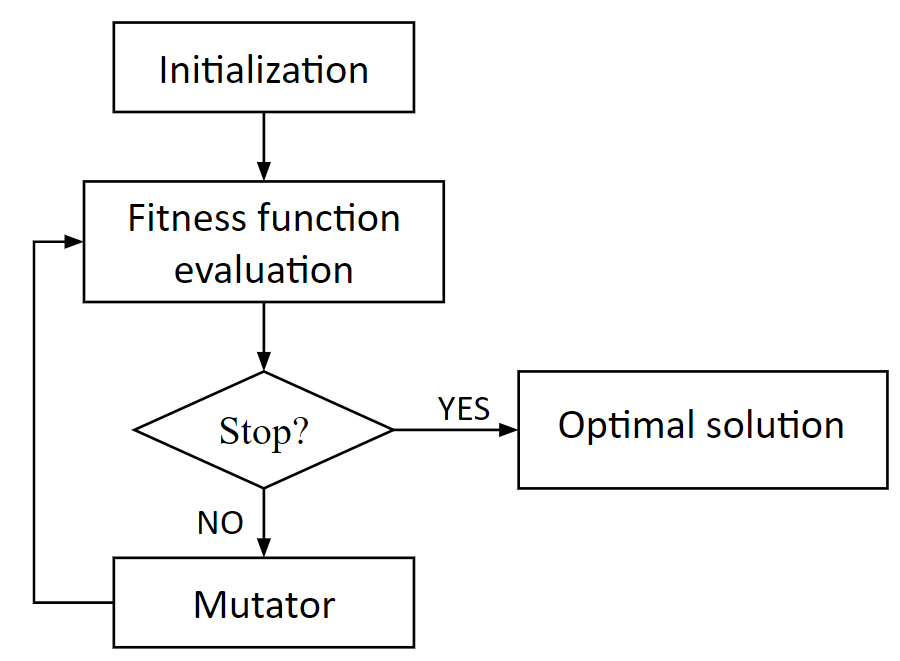
\includegraphics[width=.5\textwidth]{img/Genetic_Improvement_.png}
  \caption{Overall process of genetic improvement}
  \label{fig:Genetic_improvement_process}
\end{figure}


%Researchers have already shown that GI can improve human-written code, ranging from program repair to optimizing run-time, from reducing energy consumption to the transplantation of new functionality~\cite{DBLP:conf/gecco/BrownleePABWW19}.

\vspace{.5em}

%Numerous research studies have been conducted in the Genetic improvement domain.
%
%In Table \ref{tab:Genetic Improvement Research Papers Summary} below, we present a compilation of relevant research works that are well-suited for supporting and enhancing our own research exploration. The table includes key information about each work, such as title, author name, and key findings.

\cite{DBLP:journals/tec/PetkeHHLWW18} presents a comprehensive survey of  
%the nascent field of research 
research studies on GI that were published between 1995 and 2015.
%,  with a focus on the core papers in the area published between 1995 and 2015. 
Authors identified 
%core publications including empirical studies, 
that 96\% of these studies use evolutionary algorithms (in particular genetic programming). Moreover, GI has resulted in performance improvements for a diverse set of properties such as execution time and memory consumption, as well as results for fixing and extending existing system functionality. However, only three studies focused on reducing energy consumption were mentioned in this survey. These studies are described as follows:

\begin{itemize}
    \item \cite{DBLP:conf/gecco/BrucePH15} applied GI to the \textit{MiniSAT Boolean Satisfiability} solver when specializing for three downstream applications and found that GI can successfully be used to reduce energy consumption by up to 25\%.
    
    \item \cite{DBLP:conf/gecco/MrazekVS15} presented a method based on \textit{Cartesian genetic programming} that is evaluated in the task of approximation of 9-input and 25-input median function. Resulting approximations shown a significant improvement in the execution time and power consumption with respect to the accurate median function while the observed errors are moderate.
    
    \item \cite{DBLP:conf/ssbse/BurlesBBKSV15} used a \textit{metaheuristic search} to improve Google’s Guava library by finding a semantically equivalent version of \texttt{com.google.common.collect.ImmutableMultimap} with reduced energy consumption. Semantics-preserving transformations were found in the source code using the principle of subtype polymorphism. A new tool, \texttt{Opacitor}, was introduced to deterministically measure energy consumption and it was found that a statistically significant reduction to Guava’s energy consumption is possible. 
\end{itemize}


%{\footnotesize
%\begin{longtable}{|p{4.3cm}|p{3.2cm}|p{8.5cm}|}

%  \hline
%  \textbf{Title} & \textbf{Author Name} & \textbf{Key Findings}\\
  
%  \hline
%  Genetic Improvement of Software: A Comprehensive Survey ~\cite{DBLP:journals/tec/PetkeHHLWW18} & 
%  Justyna Petke, Saemundur O. Haraldsson, Mark Harman, William B. Langdon, David R. White, and John R. &
%  Present a comprehensive survey of the nascent field of research on Genetic Improvement (GI) with a focus on the core papers in the area published between 1995 and 2015. Authors identified core publications including empirical studies, 96\% of which use evolutionary algorithms (genetic programming in particular). GI has resulted in performance improvements for a diverse set of properties such as execution time, energy and memory consumption, as well as results for fixing and extending existing system functionality.\\
   
%  \hline
%   Gin: Genetic Improvement Research Made Easy ~\cite{DBLP:conf/gecco/BrownleePABWW19} & 
%   Alexander E.I. Brownlee, Justyna Petke, Brad Alexander, Earl T. Barr, Markus Wagner, and David R. &
%   Introduced an extensible and modifiable GIN toolbox for GI experimentation, with a novel combination of features. Instantiated in Java and targeting the Java ecosystem, Gin automatically transforms, builds, and tests Java projects and supports automated test generation and source code profiling. The study showed through examples and a case study how Gin facilitates experimentation and can speed up innovation in GI.\\
   
%   \hline
%   Evaluation of Genetic Improvement Tools for Improvement of Non-functional Properties of Software ~\cite{DBLP:conf/gecco/ZuoBP22} &
%   Shengjie Zuo, Aymeric Blot, Justyna Petke &
%   The study conducted a literature review of available GI tools and ran multiple experiments on the found open-source tools to examine their usability. It applied a cross-testing strategy to check whether the available tools can work on different programs. Overall, the study found 63 GI papers that use a GI tool to improve non-functional properties of software, out of which 31 are accompanied by open-source code. The study was able to successfully run eight GI tools and found that ultimately only two, Gin, and PyGGI, can be readily applied to new general software.\\
   
%   \hline
%   Multi-Objective Genetic Improvement: A Case Study with EvoSuite ~\cite{DBLP:conf/ssbse/CallanP22} & 
%   James Callan and Justyna Petke &
%   Present an extension of an existing generalist, open-source genetic improvement tool, Gin, with a multi-objective search strategy, NSGA-II. The implementation was conducted on a mature, large software, EvoSuite, a tool for automatic test case generation for Java. The multi-objective extension of Gin was utilized to improve both the execution time and memory usage of EvoSuite. The study found improvements in the execution time of up to 77.8\% and improvements in memory usage of up to 9.2\% on the mentioned test set.\\
   
%   \hline
%   Reducing Energy Consumption Using Genetic Improvement ~\cite{DBLP:conf/gecco/BrucePH15} &
%   Bobby R. Bruce,\kern0.2em Justyna Petke and Mark Harman &
%   Applied GI to the MiniSAT Boolean satisfiability solver when specializing for three downstream applications and found that GI can successfully be used to reduce energy consumption by up to 25\%.\\
   
%   \hline
%    Evolutionary Approximation of Software for Embedded Systems: Median Function ~\cite{DBLP:conf/gecco/MrazekVS15} &
%    Vojtech Mrazek, Zdenek Vasicek, Lukas Sekanina &
%    The study presented a method based on Cartesian genetic programming that is evaluated in the task of approximation of 9-input and 25-input median function. Resulting approximations shown a significant improvement in the execution time and power consumption with respect to the accurate median function while the observed errors are moderate. \\
   
%   \hline
%    Object-Oriented Genetic Improvement for Improved Energy Consumption in Google Guav ~\cite{DBLP:conf/ssbse/BurlesBBKSV15} &
%    Nathan Burles, Edward Bowles, Alexander E. I. Brownlee, Zoltan A. Kocsis, Jerry Swan and Nadarajen Veerapen &
%    In this study, the authors used a metaheuristic search to improve Google’s Guava library by finding a semantically equivalent version of com.google.common.collect.ImmutableMultimap with reduced energy consumption. Semantics-preserving transformations were found in the source code using the principle of subtype polymorphism. A new tool, Opacitor, was introduced to deterministically measure energy consumption and it was found that a statistically significant reduction to Guava’s energy consumption is possible. \\
%   \hline
%\caption{Genetic Improvement Research Papers Summary}
%\label{tab:Genetic Improvement Research Papers Summary}
%\end{longtable}
%}

After a thorough analysis of existing research work on GI, it becomes evident that GI is a powerful technique that can be used to automatically find improved versions of existing software with respect to various non-functional properties such as execution time, energy consumption, memory usage, etc. Several tools have been developed to facilitate experimentation with GI, including \textit{Gin} and \textit{PyGGI}. These tools have been successfully applied to various software systems, resulting in significant improvements in performance. 

%In the subsequent subsection \ref{sub:Justify the selection of the Gin Tool for the improvement of non-functional properties of software}, we will discuss about the selection of Gin tool and justify why this tool will be suitable for our work. 

%\subsection{Justify the selection of the Gin Tool for the improvement of non-functional properties of software}

%\label{sub:Justify the selection of the Gin Tool for the improvement of non-functional properties of software}
\vspace{.5em}
\cite{DBLP:conf/gecco/ZuoBP22} conducted a literature review of available GI tools and ran multiple experiments on the found open-source tools to examine their usability. It applied a cross-testing strategy to check whether the available tools can work on different programs. The study found 63 GI papers that introduce a GI tool to improve non-functional properties of software, out of which 31 are accompanied by open-source code. From these tools, the study was able to successfully run 8 GI tools.
%and found that ultimately only two, Gin, and PyGGI, can be readily applied to new general software.
%According to~\cite{DBLP:conf/gecco/ZuoBP22}, the authors found 63 papers that introduced a GI tool to improve non-functional properties of software, of which 31 introduced open-source codes,
%The usability study of this research exposed 11 different general GI tools, 
%but only 8 were able to run without any issues. Furthermore, %the generalizability study of this research ultimately showed that 
Among these 8 GI tools, only 2, \ie Gin and PyGGI, can be readily applied to new software for the improvement of non-functional properties. The Gin tool\footnote{\url{https://github.com/gintool/gin}} provides an extensible and modifiable toolbox for GI experimentation, specifically targeting the Java ecosystem. 
%On the other hand, 
The PyGGI tool\footnote{\url{https://github.com/coinse/pyggi}} offers a Python General lightweight and simple framework for Genetic Improvement. In the subsequent section we will discuss about Gin tool. 

\vspace{.5em}
As mentioned in Section \ref{sec:problem_statement} of Chapter \ref{ch:Introduction}, we selected the Java programming language as our primary focus for our research work because it spends less energy than other programming languages such as Python. Therefore, 
%we preferred a Java-based Genetic Improvement tool instead of a Python-based Genetic Improvement tool. That's why 
we selected the Gin tool, a Java-based Genetic Improvement tool, to help us improve non-functional properties of software with the objective of reducing energy consumption. 
%In the subsequent subsection \ref{subsection:Gin_Tool} we will discuss about Gin Tool. 

\subsection{The Gin Toolbox}
\label{subsection:Gin_Tool}

%Introduced an extensible and modifiable GIN toolbox for GI experimentation, with a novel combination of features. Instantiated in Java and targeting the Java ecosystem, Gin automatically transforms, builds, and tests Java projects and supports automated test generation and source code profiling. The study showed through examples and a case study how Gin facilitates experimentation and can speed up innovation in GI.

Gin~\cite{DBLP:conf/gecco/BrownleePABWW19} is a GI tool that aims to facilitate experimentation and research in the field of software development. It provides an extensible and modifiable toolbox for GI experimentation, specifically targeting the Java ecosystem. By automating the transformation, building, and testing of Java projects, Gin supports various aspects of software improvement, including program repair, run-time optimization, energy consumption reduction, and the addition of new functionality. 

\vspace{.5em}
In a recent work~\cite{DBLP:conf/ssbse/CallanP22},  
an extension of the Gin toolbox was presented.
%, open-source genetic improvement tool, 
Gin was extended with a multi-objective search algorithm, \ie NSGA-II. 
%The implementation was conducted on a mature, large software, EvoSuite, a tool for automatic test case generation for Java. 
The multi-objective extension of Gin was utilized to improve both the execution time and memory usage of EvoSuite as case study. The study found improvements in the execution time of up to 77.8\% and improvements in memory usage of up to 9.2\% on the mentioned test set.

\vspace{.5em}
Gin incorporates features such as automated test generation and source code profiling, which are essential for non-functional improvement. Gin's design focuses on scalability, allowing it to handle large-scale systems and integrate with popular Java build systems like Maven and Gradle. It supports multiple representations of code, providing flexibility for researchers to define custom mutation operators and transformation strategies. Additionally, Gin introduces innovative features for non-functional improvement, including built-in profiling and automated test case generation.\par


\begin{figure}[h]
  \centering
  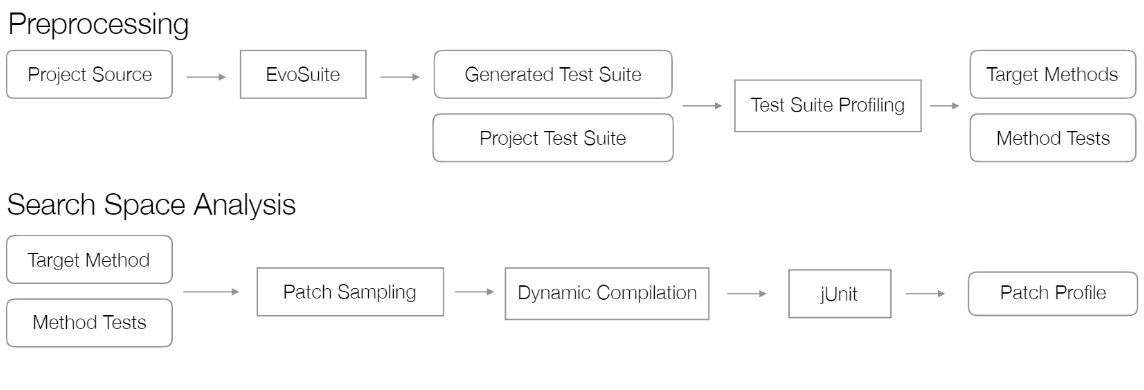
\includegraphics[width=1.0\textwidth]{img/Gin_Pipelines.png}
  \caption{Gin Pipelines from~\cite{DBLP:conf/gecco/BrownleePABWW19}}
  \label{fig:GinPipelines}
\end{figure}


As shown in Figure~\ref{fig:GinPipelines}, Gin provides two pipelines: \textit{Preprocessing} and \textit{Search Space Analysis}:\par

\vspace{.5em}
\textbf{Preprocessing}: Gin can preprocess a project and find the methods that are most likely to benefit from genetic improvement (GI). This is done by using the gin.util.Profiler class, which measures the execution time of each method in the project and ranks them by their contribution to the overall performance. The methods with the highest execution time are called 'hot methods' and are output as suitable targets for improvement by GI.\par

\vspace{.5em}
\textbf{Search Space Analysis}: Gin can also help to analyze the search space of possible program edits that can be applied by GI. The toolkit provides several tools that can sample and enumerate different types of edits, such as statement deletion, insertion, or replacement. These tools can be easily extended or reused to add new edit types. Gin will test each sampled or enumerated edit by applying it to the original code and running a test suite against the modified code. Gin will record various information about each edit, such as its validity (whether it preserves the functionality of the original code), its compilation result, its test output (whether it passes or fails the test suite), its run time (how long it takes to execute the test suite), and its error details (if any). Gin can use any test suite that is in JUnit format, which is a widely used testing framework for Java. Gin can also capture more detailed test output than just pass or fail, such as the difference between the expected and actual output. This allows Gin to support more fine-grained fitness functions that can measure the quality of each edit more accurately.\par


\begin{figure}[h]
  \centering
  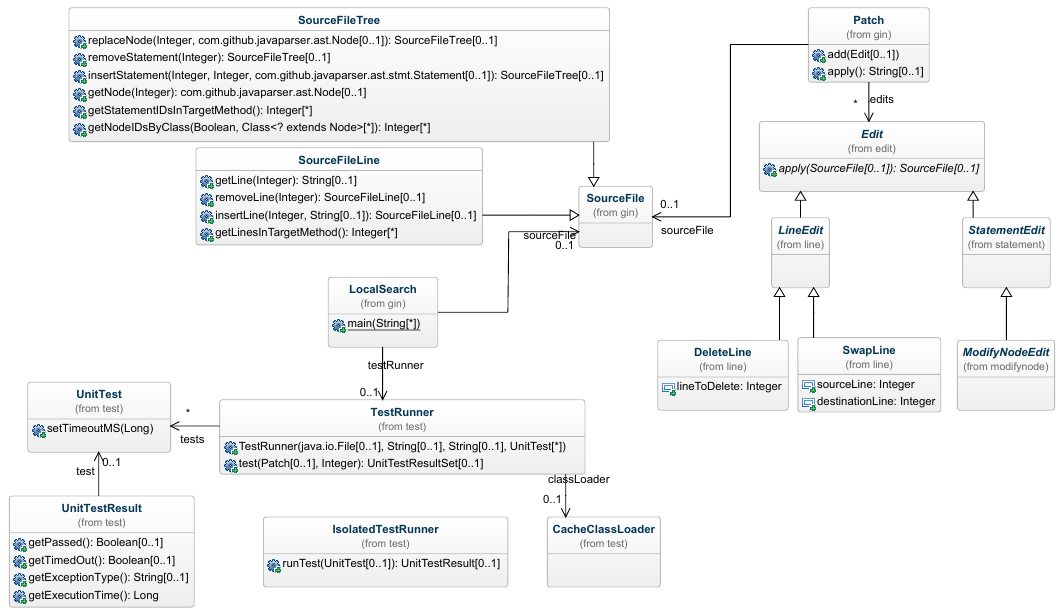
\includegraphics[width=.9\textwidth]{img/Ginclass.png}
  \caption{Gin Core Classes from~\cite{DBLP:conf/gecco/BrownleePABWW19}}
  \label{fig:Gin_Core_Classes}
\end{figure}

The Gin toolkit encompasses a collection of classes mentioned in Figure \ref{fig:Gin_Core_Classes} designed to facilitate genetic improvement research by offering a framework for manipulating source code, executing tests, and analyzing outcomes. At the core of this toolkit lies the SourceFile class, an immutable representation of the original source code, equipped with various methods for modifying the codebase, accessing language constructs, and generating modified Java source code.\par

\vspace{.5em}
Derived from the SourceFile class, the SourceFileTree subclass focuses on edits to the Abstract Syntax Tree (AST) of the source code. It assigns unique identifiers to each node within the AST, enabling efficient resolution of patches that entail multiple edits to the same location. In a similar vein, the SourceFileLine subclass directs its attention to line-level edits, also employing unique IDs for each line to simplify edit application.\par

\vspace{.5em}
A crucial component within Gin is the Patch class, which serves as a container for a series of edits, encapsulating the desired changes to be applied to the source code. The Edit class, serving as the base class for different types of edits, represents the application of a specific operator to the target source code. Subclasses of Edit, including LineEdit and StatementEdit, offer a range of operations for manipulating lines of code and modifying statements, respectively. The granularity of these edits provides fine-grained control over the code transformations.\par

\vspace{.5em}
To explore the search space of software transformations, the LocalSearch class employs a combination of sampling and searching techniques. It navigates through possible modifications to improve the code, ultimately enhancing its quality and performance. Meanwhile, the TestRunner class utilizes the JUnit framework to execute unit tests, offering insights into the outcomes, execution time, and encountered errors of the modified code.\par

\vspace{.5em}
The UnitTest class represents an individual unit test and is employed by the TestRunner to evaluate the test outcomes. Storing the result of a unit test, including pass/fail status, expected and actual results, and error details, the UnitTestResult class aids in analyzing the impact of code modifications on test behavior.\par

\vspace{.5em}
For focused testing of individual edits or patches, the IsolatedTestRunner subclass of TestRunner conducts tests in isolation. Finally, the CatcheClassLoader class, a custom ClassLoader, loads the modified class during test execution, overlaying the existing class hierarchy and facilitating the loading of the modified class by JUnit.\par

\vspace{.5em}
Collectively, these classes and their interplay within the Gin toolkit provide researchers with a powerful foundation for genetic improvement studies. The toolkit simplifies the process of editing source code, conducting tests, and evaluating the effects of modifications, thereby enabling more efficient and effective research in this domain. \par

\subsection{Identify the element need to be extended in the Gin tool}

In the previous subsection \ref{subsection:Gin_Tool}, we mentioned that the Gin tool comprises a collection of classes. Among these classes, the Edit class serves as the base class for different types of edits, representing the application of specific operators to the target source code. The subclasses of Edit, namely LineEdit and StatementEdit, offer a range of operations for manipulating lines of code and modifying statements, respectively. Based on the information mentioned above, it can be concluded that code refactoring techniques can be integrated into the genetic improvement tool, Gin Tool.

\begin{figure}[ht!]
  \centering
  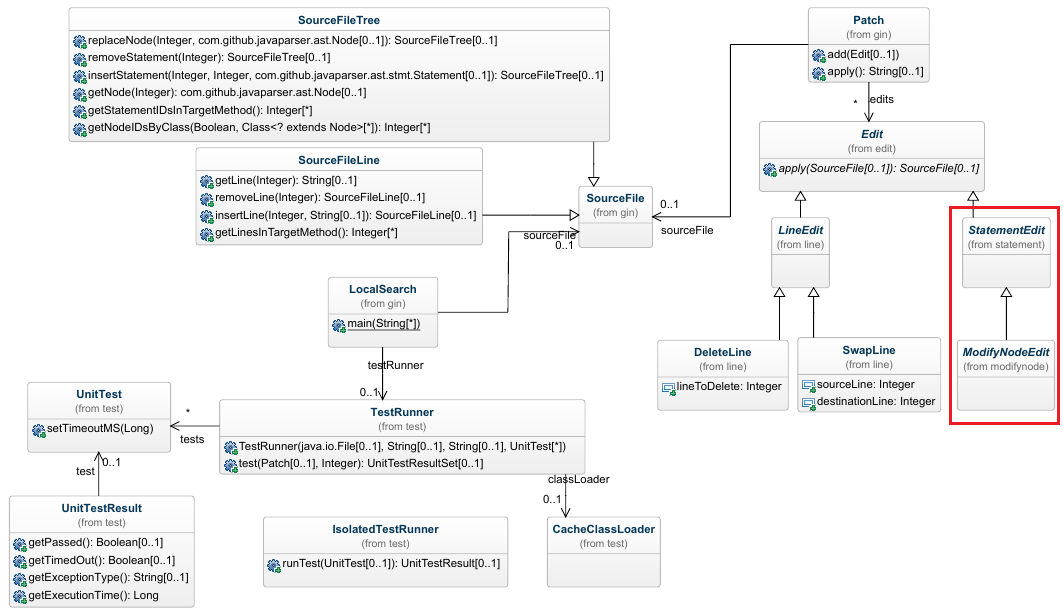
\includegraphics[width=.9\textwidth]{img/Gin_Core_Classes_extentions.png}
  \caption{Extension of the Gin Tool's class.~\cite{DBLP:conf/gecco/BrownleePABWW19}}
  \label{fig:Gin_Core_Classes_Extension}
\end{figure}

\vspace{.5em}
According to the information provided, the Edit class in the Gin tool acts as the base class for different types of edits and has two subclasses, LineEdit (providing a variety of operations for manipulating lines of code) and StatementEdit (offering a range of operations for modifying statements). Consequently, we have identified the StatementEdit class as the appropriate class for integrating selected code refactoring techniques. As StatementEdit offers a range of operations for modifying statements, and code refactoring techniques are closely related to statement edits, we consider StatementEdit to be the suitable class for incorporating code refactoring techniques. This integration will aid in obtaining the best patch, indicating an improved version of the program that consumes less energy.

\vspace{1em}
Figure \ref{fig:Gin_Core_Classes_Extension} below illustrates the identified class of the Gin tool where we will integrate the selected code refactoring techniques.



\section{Conclusion}
Through a comprehensive literature review, it has been observed that while various code refactoring techniques can improve software performance, their impact on energy efficiency varies based on the software's specific context. Notably, techniques like 'Convert Local Variable to Field', 'Introduce Parameter Object', and others have shown promise in reducing energy consumption. The Genetic Improvement (GIN) tool, which leverages Genetic Programming for software enhancement, presents an ideal platform to integrate these techniques. The StatementEdit class within GIN appears to be the most fitting for this integration, paving the way for potentially higher software quality and energy efficiency. This study effectively addresses the research question, highlighting the potential synergies between refactoring techniques and the GIN tool. Based on this analysis, we can answer research question \textbf{RQ2.2}: Code refactoring techniques can indeed be integrated into the Genetic Improvement tool, Gin. For this integration, the StatementEdit class in Gin will need to be extended. 
